


\chapter{Use of external programs}
\label{chap-external-programs}
This chapter presents the use of the different programs of which Unitex is
composed. These programs, which can be found in the \verb+Unitex/App+ directory, are
automatically called by the interface (in fact, \verb+UnitexToolLogger+ is
actually called, in order to reduce significantly the size of the downloadable
zip file). It is possible to see the commands that have been executed by
clicking on "Info>Console". It is also possible to see the options of the different programs on "Info>Help on commands" (see Figure \ref{fig-help}). Note that that all Unitex
programs support the \verb$-h$/\verb$--help$ option.

\bigskip
\begin{figure}[!h]
\begin{center}
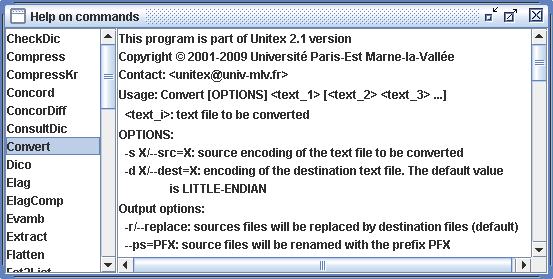
\includegraphics[width=14cm]{resources/img/fig11-1.png}
\caption{Help on commands\label{fig-help}}
\end{center}
\end{figure}

\bigskip
\noindent WARNING: many programs use the text directory\index{Directory!text}\index{Text!directory}
(\verb+my_text_snt+). This directory is created by the graphical interface after
the normalization of the text. If you work with the command line, you have to
create the directory manually before the execution of the program
\verb+Normalize+.

\bigskip
\noindent WARNING (2): whenever a parameter contains spaces, it needs to
be enclosed in quotation marks so it will not be considered as multiple
parameters.
\index{External programs!\verb+Normalize+}\index{\verb+Normalize+}

\bigskip
\noindent WARNING (3): many programs need an \verb+Alphabet.txt+ file. For all
those programs, this information can be omitted. In that case, a default
definition of letters is used (see \verb+u_is_letter+ 
in \verb$Unicode.cpp$ source file).


\section{Creating log files}\index{Creating log files}
\label{section-creating-log-files}

\bigskip
\begin{figure}[!h]
\begin{center}
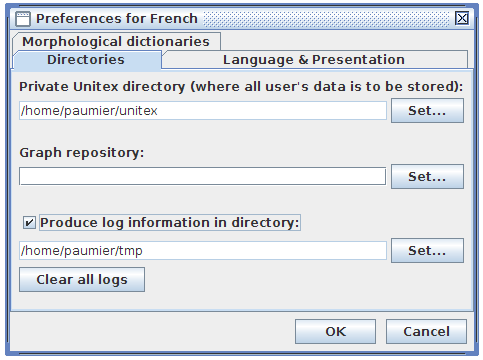
\includegraphics[width=10cm]{resources/img/fig11-1a.png}
\caption{Logging configuration\label{fig-logging-config}}
\end{center}
\end{figure}

You can create log files of external program launches. These log files can be useful for debugging
or regression tests. You just need to enable this feature in the Preferences frame. You have
to choose a log directory where all log files will be stored and to select the "Produce log"
check box. Clicking on the "Clear all logs" button will remove all log files contained in this directory,
if any. Then, any further program execution will produce a \verb+unitex_log_XXX.ulp+ file located in the log 
directory. \verb+XXX+ stands for the log number that can be found in the console (see next section).



\section{The console}\index{Console}
\label{section-console}
When Unitex launches an external program, the invoked command line is stored in
the console. To see it, click on ``Info>Console''. When a command emits
no error message, it is displayed with a green icon. Otherwise, the icon is a red
triangle that you can click on to see the error messages, as shown on Figure
\ref{fig-console}. This is useful when an error message occurs so fast that you
cannot read it. If a command has been logged, its log number appears in the second column.
Note that you can export all the commands diplayed in the
console to the clipboard with Ctrl+C.

\bigskip
\begin{figure}[!h]
\begin{center}
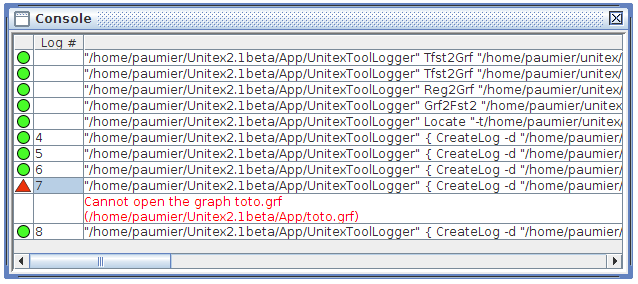
\includegraphics[width=15cm]{resources/img/fig11-2.png}
\caption{Console\label{fig-console}}
\end{center}
\end{figure}

\section{Unitex JNI}
\index{Unitex JNI}
\label{section-unitex-JNI}

You can use Unitex as a Java Native interface by including the following imports : 
\begin{verbatim}
import fr.umlv.unitex.jni.UnitexJni;
import java.io.*;
import fr.umlv.unitex.*;
\end{verbatim}
This will allow you to load .bin, .fst2 and alphabet files and to keep them in memory persistently. You use the filename created by loadPersistent* function.

\begin{verbatim}
String persistentAlphabet = UnitexJni.loadPersistentAlphabet("/.../unitex/French/Alphabet.txt");
String persistentFst2 = UnitexJni.loadPersistentFst2("/.../unitex/French/Dela/fogg-r.fst2");
String persistentDictionary = UnitexJni.loadPersistentDictionary(
		"/.../unitex/French/Dela/communesFR+.bin");
\end{verbatim}



\section{Text file encoding parameters}\index{Text!file!encoding parameters}
\label{section-text-file-encoding-parameters}
Unitex uses Unicode for text file\ref{unicode-encoding}. All program which read or write
text file share same encoding parameters. Possible format are 
utf16le-bom, utf16le-no-bom, utf16be-bom, utf16be-no-bom, utf8-bom, utf8-no-bom, 
for Unicode Big-Endian, Little-Endian and UTF-8, with or without Unicode byte order mark at the beginning of the file.
For the input format, you can specify several *-bom encoding separated by comma, but only one *-no-bom encoding.

\bigskip
\noindent \textbf{OPTIONS:}
\begin{itemize}
  \item \verb+-k=ENCODING+/\verb+--input_encoding=ENCODING+: input text file format. Can contain several value, separated by a comma;
  \item \verb+-q=ENCODING+/\verb+--output_encoding=ENCODING+: output text file format. 
\end{itemize}

By default, value are \verb+--input_encoding=utf16le-bom,utf16be-bom,utf8-bom --output_encoding=utf16le-bom+.


\section{BuildKrMwuDic}\index{External programs!\verb+BuildKrMwuDic+}\index{\verb+BuildKrMwuDic+}
\index{Generation of Korean MWU dictionary}\index{Korean MWU dictionary}
\verb+BuildKrMwuDic [OPTIONS] dic+

\bigskip
\noindent This program generates a MWU dictionary graph from a text table \verb+dic+ describing each component
of each MWU.  

\bigskip
\noindent \textbf{OPTIONS:}
\begin{itemize}
   \item \verb+-o GRF+/\verb+--output=GRF+: .grf file to produce;
   \item \verb+-d DIR+/\verb+--directory=DIR+: inflection directory containing the inflection graphs required
   to produce morphological variants of roots;
   \item \verb+-a ALPH+/\verb+--alphabet=ALPH+: alphabet file to use;
   \item \verb+-b BIN+/\verb+--binary=BIN+: .bin simple word dictionary to use.
\end{itemize}

\section{Cassys}\index{External programs!\verb+Cassys+}\index{\verb+Cassys+}
\index{Cascade of transducers}
\verb+Cassys [OPTIONS] <snt>+

\bigskip
\noindent This program applies an ordered list of grammars to a text and constructs an index of the occurrences found.

\bigskip
\noindent \textbf{OPTIONS:}
\begin{itemize}
  \item \verb+-a ALPH+/\verb+--alphabet=ALPH+: the language alphabet file
  \item \verb+-r X+/\verb+--transducer_dir=X+: take tranducer on directory X (so you don't specify full path for each transducer; note that X must be (back)slash terminated
	\item \verb+-l TRANSDUCERS_LIST+/\verb+--transducers_list=TRANSDUCERS_LIST+: the transducers list file with their output policy
	\item \verb+-s transducer.fst2+/\verb+--transducer_file=transducer.fst2+: a transducer to apply
	\item \verb+-m output_policy+/\verb+--transducer_policy=output_policy+: the output policy of the transducer specified
%//// -f FILE/--file=FILE: the snt text file
  \item \verb+-t TXT+/\verb+--text=TXT+: the text file to be modified, with extension .snt;
	\item \verb+-i+/\verb+--in_place+: mean uses the same csc/snt directories for each transducer
	\item \verb+-d+/\verb+--no_create_directory+: mean the all snt/csc directories already exist and don't need to be created
	\item \verb+-g minus+/\verb+--negation_operator=minus+: uses minus as negation operator for Unitex 2.0 graphs
	\item \verb+-g tilde+/\verb+--negation_operator=tilde+: uses tilde as negation operator (default)
	\item \verb+-h+/\verb+--help+: display this help
\end{itemize} 	

\bigskip
\noindent Cassys applies a list of grammar to a text and saves the matching sequence index in a file named \"concord.ind\" stored in the text directory.
      The target text file has to be a preprocessed snt file with its \_snt/ directory. 
      The transducer list file is a file in which each line contains the path to a transducer followed by the output policy to be applied to this transducer.

\bigskip
\noindent Instead a list file, you can specify each file and each output policy by a set of couple of -s/--transducer\_file 
      and -m/--transducer\_policy argument to enumerate the list
      
\bigskip
\noindent The policy may be MERGE or REPLACE.
      
\bigskip
\noindent The file option, the alphabet option and the transducer list file option are mandatory
     
\bigskip
\noindent As the locate pattern program, this program saves the references to the found occurrences in a file called concord.ind stored 
		in the \_snt directory of the text.
		The file concord.ind produced is in the same format as described in the chapter \ref{chap-file-formats} , but the cascade may be constituted of graphs 
applied in merge or replace mode so the \#M or \#R at the first line of the file concord.ind has no sense in this context.



\section{CheckDic}\index{External programs!\verb+CheckDic+}\index{\verb+CheckDic+}
\index{Verification of the dictionary format}\index{Dictionaries!verification}
\verb+CheckDic [OPTIONS] dic+

\bigskip
\noindent This program carries out the verification of the format of a dictionary
of DELAS or DELAF type. \verb+dic+ corresponds to the name
of the dictionary that is to be verified. 

\bigskip
\noindent \textbf{OPTIONS:}
\begin{itemize}
  \item \verb+-f+/\verb+--delaf+: checks an inflected dictionary;
  \item \verb+-s+/\verb+--delas+: checks a non inflected dictionary;
  \item \verb+-r+/\verb+--strict+: strict syntax checking against unprotected dot and comma;
  \item \verb+-t+/\verb+--tolerate+: tolerates unprotected dot and comma (default);
  \item \verb+-n+/\verb+--no_space_warning+: tolerates spaces in
  grammatical/semantic/inflectional codes;
  \item \verb+-p+/\verb+--skip_path+: does not display the full path of the dictionary (useful 
  for consistent log files across several systems);
  \item \verb+-a ALPH+/\verb+--alphabet=ALPH+: specifies the alphabet file to
        use. 
        
\end{itemize}

\bigskip
\noindent The program checks the syntax of the lines of the dictionary. It also creates a
list of all characters occurring in the inflected and canonical forms of words in
the text, the list of grammatical codes and syntax, as well as the list of
inflection codes used. The results of the verification are stored in a file
called \verb+CHECK_DIC.TXT+.\index{File!\verb+CHECK_DIC.TXT+}

\bigskip
\noindent Selecting strict syntax checking detects using unprotected dot in
inflected form, or unprotected comma in lemma. The \verb+--tolerate+ option acts like Unitex 2.0
and lower and does not detect them.





\section{Compress}\index{External programs!\verb+Compress+}\index{\verb+Compress+}
\index{Compression of a dictionary}
\label{section-compress}
\verb+Compress [OPTIONS] dictionary+
\index{Dictionaries!DELAF}\index{Dictionaries!compression}
\index{File!\verb+.dic+}\index{File!\verb+.bin+}\index{File!\verb+.inf+}

\bigskip
\noindent \textbf{OPTIONS:}
\begin{itemize}
  \item \verb+-o BIN+/\verb+--output=BIN+: sets the output file. By default, a file \verb+xxx.dic+ will
  produce a file \verb+xxx.bin+;
  \item \verb+-f+/\verb+--flip+: indicates
  that the inflected and canonical forms should be swapped in the compressed
  dictionary. This option is used to construct an inverse dictionary which is
  necessary for the program \verb+Reconstrucao+;
  \item \verb+-s+/\verb+--semitic+: indicates that the semitic compression algorithm should be used. Setting
  this option with semitic languages like Arabic significantly reduces the size of the output dictionary.
  \item \verb+--v1+: produces an old style .bin file
  \item \verb+--v2+: produces a new style .bin file, with no file size limitation to 16 Mb and 
  a smaller size (default)
\end{itemize}

\bigskip
\noindent This program takes a DELAF dictionary as a parameter and compresses it.
The compression of a dictionary \verb+dico.dic+ produces two files:
\begin{itemize}
  \item \verb+dico.bin+: a binary file containing the minimum automaton of the inflected forms of the dictionary;
  \item \verb+dico.inf+: a text file containing the compressed forms required for the reconstruction of the dictionary
  lines from the inflected forms contained in the automaton.
\end{itemize}

\bigskip
\noindent For more details on the format of these files, see chapter
\ref{chap-file-formats}.






\section{Concord}\index{External programs!\verb+Concord+}\index{\verb+Concord+}\index{Concordance}
\label{section-Concord}
\index{Text!modification}\index{Modification of the text}
\verb+Concord [OPTIONS] <index>+

\bigskip
\noindent This program takes a concordance index file produced by the program
\verb+Locate+ and produces a concordance. It is also possible to produce a
modified text version taking into account the transducer outputs associated to
the occurrences. Here is the description of the parameters:

\bigskip
\noindent \textbf{OPTIONS:}
\begin{itemize}
  \item \verb+-f FONT+/\verb+--font=FONT+: the name of the font to use if the
  output is an HTML file;
  \item \verb+-s N+/\verb+--fontsize=N+: the font size to use if the output is
  an HTML file. The font parameters are required if the output is an HTML file;
  \item \verb+--only_ambiguous+: Only displays identical occurrences with 
  ambiguous outputs, in text order.
  \item \verb+--only_matches+: this option will force empty right and left contexts.
  Moreover, if used with -t/--text, Concord will not surround matches with tabulations
  \item \verb+-l X+/\verb+--left=X+: number of characters on the left of the 
  occurrences (default=0). In Thai mode, this means the number of non-diacritic
  characters.\index{Contexts!concordance}
  \item \verb+-r X+/\verb+--right=X+: number of characters (non-diacritic ones in Thai mode) on
  the right of the occurrences (default=0). If the occurrence is shorter than
  this value, the concordance line is completed up to \verb+right+. If the occurrence is longer
  than the length defined by \verb+right+, it is nevertheless saved as whole.
  
  \bigskip
  NOTE: For both \verb+--left+ and \verb+--right+, you can add the \verb+s+
  character to stop at the first \verb+{S}+ tag. For instance, if you
  set \verb+40s+ for the left value, the left context will end at 40 characters
  at most, less if the \verb+{S}+ tag is found before.
\end{itemize}

\bigskip
\noindent \textbf{Sort order options:}\index{Sorting!concordances}
\begin{itemize}
  \item \verb+--TO+: order in which the occurrences appear in the text
  (default);
  \item \verb+--LC+: left context for primary sort, then occurrence for
    secondary sort;
  \item \verb+--LR+: left context, then right context;
  \item \verb+--CL+: occurrence, then left context;
  \item \verb+--CR+: occurrence, then right context;
  \item \verb+--RL+: right context, then left context;
  \item \verb+--RC+: left context, then occurrence.
\end{itemize}
\noindent For details on the sorting modes, see section
\ref{section-display-occurrences}.

\bigskip
\noindent \textbf{Output options:}
\begin{itemize}
  \item \verb+-H+/\verb+--html+: produces a concordance in HTML format encoded in
    UTF-8\index{UTF-8} (default);
  \item \verb+-t+/\verb+--text+: produces a concordance in Unicode text format; 
  \item \verb+-g SCRIPT+/\verb+--glossanet=SCRIPT+: produces a concordance for GlossaNet
  in HTML format. The HTML file is encoded in UTF-8;\index{GlossaNet}

  \item \verb+-p SCRIPT+/\verb+--script=SCRIPT+: produces a HTML concordance
  file where occurrences are links described by \verb+SCRIPT+. For instance, if
  you use
  
  %do not remove this line jump
  \verb$-phttp://www.google.com/search?q=$, you will obtain
  a HTML concordance file where occurrences are hyperlinks to Google queries;

  \item \verb+-i+/\verb+--index+: produces an index of the concordance, made of the
    content of the occurrences (with the grammar outputs, if any), preceded by
    the positions of the occurrences in the text file given in characters;
  \item \verb+-u+ \verb+offsets+/\verb+--uima=offsets+: produces an index of the 
  concordance relative to the original text file, before any Unitex operation. Offsets 
  is supposed to be the file produced by Tokenize's \verb+--output_offsets+ option
%  the same as \verb+--index+, but the ending position of each occurrence is also given;
  \item \verb+--PRLG=X,Y+: produces a concordance for PRLG corpora where each line
  is prefixed by information extracted with Unxmlize's \verb+--PRLG+ option. X is the 
  file produced by Unxmlize's \verb+--PRLG+ option and Y is the file produced by Tokenize's
  \verb+--output_offsets+ option. Note that if this option is used in addition with \verb+-u+, 
  the Y argument oferrides the argument of \verb+-u+;
  \item \verb+-e+/\verb+--xml+: produces xml index of the concordance;
  \item \verb+-w+/\verb+--xml-with-header+: produces xml index of the concordance with full xml header;
  \item \verb+-A+/\verb+--axis+: quite the same as \verb+--index+, but the numbers
    represent the median character of each occurrence. Fore more information,
    see \cite{axis};
  \item \verb+-x+/\verb+--xalign+: another index file, used by the text alignment module.
    Each line is made of 3 integers $X$ $Y$ $Z$ followed by the content of the 
    occurrence. $X$ is the sentence number, starting from 1. $Y$ and $Z$ are the
    starting and ending positions of the occurrence in the sentence, given in
    characters;
  \item \verb+-m TXT+/\verb+--merge=TXT+: indicates to the program that it is supposed to
    produce a modified version of the text and save it in a file named
    \verb+TXT+ (see section \ref{section-modifying-text}).
\end{itemize}

\bigskip
\noindent \textbf{Other options:}
\begin{itemize}
  \item \verb+-d DIR+/\verb+--directory=DIR+: indicates to the program that
  it must not work in the same directory than \verb+<index>+ but in \verb+DIR+;
  \item \verb+-a ALPH+/\verb+--alphabet=ALPH+: alphabet file used for sorting;
  \item \verb+-T+/\verb+--thai+: option to use for Thai concordances.
  \index{Alphabet}\index{File!alphabet}
\end{itemize}

\index{File!\verb+.html+}\index{File!\verb+.txt+}
\bigskip
\noindent The result of the application of this program is a file called \verb+concord.txt+
if the concordance was constructed in text mode, a file called
\verb+concord.html+ if the output mode was \verb+--html+, \verb+--glossanet+ or
\verb$--script$, and a text file with the name defined by the user of the program 
if the program has constructed a modified version of the text.

\bigskip
\noindent In \verb+--html+ mode, the occurrence is coded as a hypertext link. The reference
associated to this link is of the form \verb+<a href="X Y Z">+. \verb+X+ et
\verb+Y+ represent the beginning and ending positions of the occurrence in
characters in the file \verb+text_name.snt+. \verb+Z+ represents the number of
the sentence in which the occurrence was found.






\section{ConcorDiff}\index{External programs!\verb+ConcorDiff+}\index{\verb+ConcorDiff+}
\verb+ConcorDiff [OPTIONS] <concor1> <concor2>+

\bigskip
\noindent This program takes two concordance files and produces an HTML page
that shows their differences (see section
\ref{section-comparing-concordances}, page \pageref{section-comparing-concordances}). 
\verb+<concor1>+ and \verb+<concor2>+ concordance index files must 
have absolute names, because Unitex uses these names to deduce on which text
there were computed.

\bigskip
\noindent \textbf{OPTIONS:}
\begin{itemize}
  \item \verb+-o X+/\verb+--out=X+: output HTML page;
  \item \verb+-f FONT+/\verb+--font=FONT+: name of the font to use in output
  HTML page;
  \item \verb+-s N+/\verb+--size=N+: font size to use in output HTML page.
  \item \verb+-d/--diff_only+: don't show identical sequences;
\end{itemize}







\section{Convert}\index{External programs!\verb+Convert+}\index{\verb+Convert+}
\verb+Convert [OPTIONS] <text_1> [<text_2> <text_3> ...]+

\index{Unicode}
\bigskip
\noindent With this program you can transcode text files.

\bigskip
\noindent \textbf{OPTIONS:}
\begin{itemize}
  \item \verb+-s X+/\verb+--src=X+: input encoding;
  \item \verb+-d X+/\verb+--dest=X+: output encoding
  (default=\verb$LITTLE-ENDIAN$);
\end{itemize}

\bigskip
\noindent \textbf{Transliteration options (only for Arabic):}
\begin{itemize}
  \item \verb+-F+/\verb+--delaf+: the input is a DELAF and we only want to transliterate the inflected form and the lemma;
  \item \verb+-S+/\verb+--delas+: the input is a DELAS and we only want to transliterate the lemma.
\end{itemize}


\bigskip
\noindent \textbf{Output options:}
\begin{itemize}
  \item \verb+-r+/\verb+--replace+: input files are overwritten (default);
  \item \verb+-o file+/\verb+--output=file+: name of destination file (only one file to convert);
  \item \verb+--ps=PFX+: input files are renamed with the \verb+PFX+ prefix
        (\verb+toto.txt+ $\Rightarrow$ \verb+PFXtoto.txt+);
  \item \verb+--pd=PFX+: ouput files are renamed with the \verb+PFX+ prefix;
  \item \verb+--ss=SFX+: input files are named with the \verb+SFX+ suffix;
        (\verb+toto.txt+ $\Rightarrow$ \verb+totoSFX.txt+);
  \item \verb+--sd=SFX+: ouput files are named with the \verb+SFX+ suffix.
\end{itemize}

\bigskip
\noindent \textbf{HTML options:}

\noindent \verb+Convert+ offers some special options dedicated to HTML files. You can 
use a combination of the following options:

\begin{itemize}
  \item \verb+--dnc+ (Decode Normal Chars): things like \verb+&eacute;+
  \verb+&#120;+ and \verb+&#xF8;+ will be decoded as the single equivalent 
  unicode character, except if it represents an HTML control character;
  
  \item \verb+--dcc+ (Decode Control Chars): \verb+&lt;+ \verb+&gt;+
  \verb+&amp;+ and \verb+&quot;+ will be decoded as \verb+<+ \verb+>+
  \verb+&+ and the quote (the same for their decimal and hexadecimal
  representations);
  
  \item \verb+--eac+ (Encode All Chars): every character that is not supported by
  the output encoding will be encoded as a string like \verb+&#457;+
  
  \item \verb+--ecc+ (Encode Control Chars): \verb+<+ \verb+>+
  \verb+&+ and the quote will be encoded by \verb+&lt;+ \verb+&gt;+
  \verb+&amp;+ and \verb+&quot;+
\end{itemize} 

\noindent All HTML options are deactivated by default.

\bigskip
\noindent \textbf{Other options:}
\begin{itemize}
  \item \verb+-m+/\verb+--main-names+: prints the list of the encoding main
  names;
  \item \verb+-a+/\verb+--aliases+: prints the list of the encoding aliases;
  \item \verb+-A+/\verb+--all-infos+: prints all the information about all the
  encodings;
  \item \verb+-i X+/\verb+--info=X+: prints all the information about the
  encoding X.
\end{itemize}

\bigskip
\noindent The encodings can take values in the following list (non exhaustive,
see below):

\bigskip
\verb$FRENCH$

\verb$ENGLISH$

\verb$GREEK$

\verb$THAI$

\verb$CZECH$

\verb$GERMAN$

\verb$SPANISH$

\verb$PORTUGUESE$

\verb$ITALIAN$

\verb$NORWEGIAN$

\verb$LATIN$ (default latin code page)

\verb$windows-1252$: Microsoft Windows 1252 - Latin I (Western Europe \& USA)

\verb$windows-1250$: Microsoft Windows 1250 - Central Europe

\verb$windows-1257$: Microsoft Windows 1257 - Baltic

\verb$windows-1251$: Microsoft Windows 1251 - Cyrillic

\verb$windows-1254$: Microsoft Windows 1254 - Turkish

\verb$windows-1258$: Microsoft Windows 1258 - Viet Nam

\verb$iso-8859-1  $: ISO 8859-1  - Latin 1 (Europe de l'ouest \& USA)

\verb$iso-8859-15 $: ISO 8859-15 - Latin 9 (Western Europe \& USA)

\verb$iso-8859-2  $: ISO 8859-2  - Latin 2 (Eastern and Central Europe)

\verb$iso-8859-3  $: ISO 8859-3  - Latin 3 (Southern Europe)

\verb$iso-8859-4  $: ISO 8859-4  - Latin 4 (Northern Europe)

\verb$iso-8859-5  $: ISO 8859-5  - Cyrillic

\verb$iso-8859-7  $: ISO 8859-7  - Greek

\verb$iso-8859-9  $: ISO 8859-9  - Latin 5 (Turkish)

\verb$iso-8859-10 $: ISO 8859-10 - Latin 6 (Nordic)

\verb$next-step   $: NextStep code page

\verb$LITTLE-ENDIAN$

\verb$BIG-ENDIAN$

\verb$UTF8$







\section{Dico}\index{External programs!\verb+Dico+}\index{\verb+Dico+}
\index{Dictionaries!applying}
\verb+Dico [OPTIONS] <dic_1> [<dic_2> <dic_3>...]+

\bigskip
\noindent This program applies dictionaries to a text. The text must have been cut up into
lexical units by the \verb+Tokenize+ program.

\bigskip
\noindent \textbf{OPTIONS:}
\begin{itemize}
  \item \verb+-t TXT+/\verb+--text=TXT+: complete \verb+.snt+ text file name;
  \item \verb+-a ALPH+/\verb+--alphabet=ALPH+: the alphabet file to use;
  \item \verb+-m DICS+/\verb+--morpho=DICS+: this optional parameter indicates
  which morphological-mode dictionaries are to be used, if needed by some \verb+.fst2+
  dictionaries. \verb+DICS+ represents a list of \verb+.bin+ files (with full
  paths) separated with semi-colons;
  \item \verb+-K+/\verb+--korean+: tells \verb$Dico$ that it works on Korean;
  \item \verb+-s+/\verb+--semitic+: tells \verb$Dico$ that it works on a semitic language (needed 
  if \verb$Dico$ has to compress a dictionary);
  \item \verb+-u X+/\verb+--arabic_rules=X+: specifies the Arabic typographic rule configuration file.
  \item \verb+r X+/\verb+--raw=X+: indicates that Dico should just produce one
  output file X containing both simple and compound words, without requiring a
  text directory. If X is omitted, results are displayed on the standard output.
\end{itemize}

\bigskip
\noindent
\verb+<dic_i>+ represents the path and name of
a dictionary. The dictionary must be a \verb+.bin+ dictionary (obtained with 
the \verb+Compress+ program) or a dictionary graph in the \verb+.fst2+ format (see section
\ref{section-applying-dictionaries}, page \pageref{section-applying-dictionaries}).
\index{File!\verb+.bin+}It is possible to give priorities to the dictionaries. For details see 
section \ref{section-dictionary-priorities}.

\bigskip
\noindent The program \verb+Dico+ produces the following files, and saves
them in the directory of the text:

\begin{itemize}
  \index{File!\verb+dlf+}\index{File!\verb+dlc+}\index{File!\verb+err+}\index{File!\verb+stat_dic.n+}
  \item \verb+dlf+: dictionary of simple words in the text;
  \item \verb+dlc+: dictionary of compound words in the text;
  \item \verb+err+: list of unknown words in the text;
  \item \verb+tags_err+: unrecognized simple words that are not matched by the \verb+tags.ind+ file;
  \item \verb+tags.ind+ : sequences to be inserted in the text automaton
  (see section \ref{section-dictionary-graphs}, page \pageref{section-dictionary-graphs});
  \item \verb+stat_dic.n+: file containing the number of simple words, the number
  of compound words, and the number of unknown words in the text.
\end{itemize}

\bigskip
\noindent NOTE: Files \verb+dlf+, \verb+dlc+, \verb+err+ and \verb+tags_err+ are not sorted. Use the
program \verb+SortTxt+ to sort them.



\section{DumpOffsets}\index{External programs!\verb+DumpOffsets+}\index{\verb+DumpOffsets+}
\label{section-DumpOffsets}
\textbf{Usage:} \verb+DumpOffsets [OPTIONS] <txt>+

\bigskip
\noindent\verb+<txt>: an offset file to read+

\bigskip
\noindent DumpOffsets dump sequence offset to study them.

\bigskip
\noindent \textbf{OPTIONS:}

\begin{itemize} 	 
  \item \verb+-o X+/\verb+--old=X+: name of old file to read 	 
  \item \verb+-n X+/\verb+--new=X+: name of new file to read 	 
  \item \verb+-p X+/\verb+--output=X+: name of output dump file to write 	 
  \item \verb+-f+/\verb+--full+: dump common text additionaly
  \item \verb+-q+/\verb+--quiet+: display no message 	 
  \item \verb+-c+/\verb+--no_escape_sequence+: don't escape text sequence 	 
  \item \verb+-h+/\verb+--help+: this help 	 
\end{itemize}

\noindent Example: 
\begin{verbatim}
	 UnitexToolLogger Normalize -r .\resource\Norm.txt
	        .\work\text_file.txt 	 
	        --output_offsets .\work\text_file_offset.txt 	 
	 UnitexToolLogger DumpOffsets -o .\work\text_file_offset.txt
	        -n .\work\text_file_offset.snt 	 
	        -p .\work\dump\dump_offsets.txt .\work\text_file_offset.txt 	 
\end{verbatim}

\bigskip
\noindent \textbf{Other Usage:} \verb+DumpOffsets [-m/--merge] [OPTIONS] <txt>+

\bigskip
\noindent \verb+<txt>: an offset file to read+

\bigskip
\noindent Merge two offset file(\ref{subsection-offsets-diff}, page \pageref{subsection-offsets-diff})) produced by two successive modification of text 

\bigskip
\noindent \textbf{OPTIONS:}

\begin{itemize} 	 
  \item \verb+-o X+/\verb+--old=X+: name of old file to read 	 
  \item \verb+-n X+/\verb+--output=X+: name of output merged offset file to write
\end{itemize}

\bigskip
\noindent \textbf{Other Usage:} \verb+DumpOffsets [-v/--convert_modified_to_common] [OPTIONS] <txt>+

\bigskip
\noindent \verb+<txt>: an offset file to read+

\bigskip
\noindent Create an offset file which list offset of common string between the original and modified file. At least one size must be provided 	 

\bigskip
\noindent \textbf{OPTIONS:}
	  	 
\begin{itemize} 	 
  \item \verb+-s N+/\verb+--old_size=N+: size of original file (in characters) 	 
  \item \verb+-S N+/\verb+--new_size=N+: size of modified file (in characters) 	 
  \item \verb+-p X+/\verb+--output=X+: name of output common offset file to write 	 
  \item \verb+-h+/\verb+--help+: this help 	 
\end{itemize} 	 

\bigskip
\noindent \textbf{Other Usage:} \verb+DumpOffsets [-M/--convert_modified_to_common] [OPTIONS] <txt>+

\bigskip
\noindent \verb+<txt>: an offset file to read+

\bigskip
\noindent Create a standard modified offset file from offset of common string between the original and modified file. Both size must be provided 	 
	
\bigskip
\noindent \textbf{OPTIONS:}
	  	 
\begin{itemize} 	 
  \item \verb+-s N+/\verb+--old_size=N+: size of original file (in characters) 	 
  \item \verb+-S N+/\verb+--new_size=N+: size of modified file (in characters) 	 
  \item \verb+-p X+/\verb+--output=X+: name of output common offset file to write 	 
  \item \verb+-h+/\verb+--help+: this help 	 
\end{itemize} 	 

\bigskip
\noindent \textbf{Other Usage:} \verb+DumpOffsets -o <list_of_position_file_to_read.txt>+

\bigskip
\noindent \verb+<list_of_position_file_to_read.txt>+ is a text file with just one number (a position) at each line.

\bigskip
\noindent This will convert a list of position using the offset file. 	 
	  The created file contain the converted position at each line, with a + at the end of line if the character 	 
	  at this position is on result file, a - is it was removed. 	 
	  	 
\begin{itemize}
  \item \verb+-p <list_to_create> -T <offset_file_to_read>+
\end{itemize} 	 

\noindent Using \verb+-t+ instead \verb+-T+ will do the reverse translation 	 



\section{Elag}\index{External programs!\verb+Elag+}\index{\verb+Elag+}
\verb+Elag [OPTIONS] <tfst>+

\bigskip
\noindent This program takes a \verb+.tfst+ text automaton \verb+<tfst>+ and
applies to it ambiguity removal rules.\index{File!\verb+.tfst+}

\bigskip
\noindent \textbf{OPTIONS:}
\begin{itemize}
  \item \verb+-l LANG/--language=LANG+: ELAG configuration file for the language of the
  text;
  \item \verb+-r RULES/--rules=RULES+: rule file compiled in the \verb+.rul+
  format; \index{File!\verb+.rul+}
  \item \verb+-o OUT/--output=OUT+: output text automaton.
\end{itemize}






\section{ElagComp}\index{External programs!\verb+ElagComp+}\index{\verb+ElagComp+}
\verb+ElagComp [OPTIONS]+

\bigskip
\noindent This program compiles the ELAG grammar named \verb+GRAMMAR+, or all
the grammars specified in the \verb+RULES+ file. The result is stored in the
\verb+OUT+ file that will be used by the \verb+Elag+ program.

\bigskip
\noindent \textbf{OPTIONS:}
\begin{itemize}
  \item \verb+-r RULES+/\verb+--rules=RULES+: file listing ELAG grammars;
  \item \verb+-g GRAMMAR+/\verb+--grammar=GRAMMAR+: single ELAG grammars;
  \item \verb+-l LANG+/\verb+--language=LANG+: ELAG configuration file for the language of the grammar(s);
  \item \verb+-o OUT+/\verb+--output=OUT+: output file. By default, the output file name is 
        the same as \verb+RULES+, except for the extension that is
        \verb+.rul+.\index{File!\verb+.rul+}
\end{itemize}








\section{Evamb}\index{External programs!\verb+Evamb+}\index{\verb+Evamb+}
\verb+Evamb [OPTIONS] <tfst>+

\bigskip
\noindent This program computes an average lexical ambiguity rate on the text
automaton \verb+<tfst>+, or just on the sentence which number is specified by
\verb+N+. The results of the computation are displayed on the standard output.
The text automaton is not modified.

\bigskip
\noindent \textbf{OPTIONS:}
\begin{itemize}
  \item \verb+-o OUT+/\verb+--output=OUT+: optional output filename;
  \item \verb+-s N+/\verb+--sentence=N+: sentence number.
\end{itemize}








\section{Extract}\index{External programs!\verb+Extract+}\index{\verb+Extract+}
\verb+Extract [OPTIONS] <text>+

\bigskip
\noindent This program extracts from the given text all sentences that
contain at least one occurrence from the concordance. The parameter
\verb+<text>+ represents the complete path of the text file, without 
omitting the extension \verb+.snt+.

\bigskip
\noindent \textbf{OPTIONS:}
\begin{itemize}
  \item \verb+-y+/\verb+--yes+: extracts all sentences containing matching units
  (default);
  \item \verb+-n+/\verb+--no+: extracts all sentences that don't contain
  matching units;
  \item \verb+-o OUT+/\verb+--output=OUT+: output text file;
  \item \verb+-i X+/\verb+--index=X+: the \verb+.ind+ file that describes the
        concordance. By default, \verb+X+ is the \verb+concord.ind+ file located
        in the text directory.
\end{itemize}

\bigskip
\noindent The result file is a text file that contains all extracted sentences, one
sentence per line.







\section{Flatten}\index{External programs!\verb+Flatten+}\index{\verb+Flatten+}
\index{Graph!approximation with a finite state transducer}
\index{Approximation of a grammar with a finite state transducer}
\verb+Flatten [OPTIONS] <fst2>+

\bigskip
\noindent This program takes a \verb+.fst2+ grammar as its parameter, and tries to
transform it into a finite-state transducer. 

\bigskip
\noindent \textbf{OPTIONS:}
\begin{itemize}
  \item \verb+-f+/\verb+--fst+: the grammar is "unfolded" to the maximum depth 
  and is truncated if there are calls to
  sub-graphs. Truncated calls are replaced by void transitions. The result is a
  \verb+.fst2+ grammar that only contains a single finite-state transducer;

  \item \verb+-r+/\verb+--rtn+: calls to sub-graphs that remain
  after the transformation are left as they are. The result is therefore a
  finite-state transducer in the favorable case, and an optimized grammar
  strictly equivalent to the original grammar if not (default);

  \item \verb+-d N+/\verb+--depth=N+: maximum depth to which graph calls should 
  be unfolded. The default value is 10.
\end{itemize}







\section{Fst2Check}\index{External programs!\verb+Fst2Check+}\index{\verb+Fst2Check+}
\verb+Fst2Check [OPTIONS] <fst2>+

\bigskip
\noindent This programs checks if a .fst2 file has no error for Locate.

\bigskip
\noindent \textbf{OPTIONS:}
\begin{itemize}
  \item \verb+-y+/\verb+--loop_check+: enables error checking (loop
  detection);
  \item \verb+-n+/\verb+--no_loop_check+: disables error checking (default);
  \index{Error detection in graphs}\index{Graph!error detection}\index{Errors in graphs}
  \item \verb+-t+/\verb+--tfst_check+: checks wether the given graph can be
  considered as a valid sentence automaton or not;
  \item \verb+-e+/\verb+--no_empty_graph_warning+: no warning will be emitted
  when a graph matches the empty word. This option is used by \verb+MultiFlex+
  in order not to scare users with meaningless error messages when they design
  an inflection grammar that matches the empty word.
\end{itemize}

\bigskip
\noindent \textbf{Output options:}
\begin{itemize}
  \item \verb+-o file+/\verb+--output=file+: output file for error message;
  \item \verb+-a+/\verb+--append+: opens the message output file in append mode;
  \item \verb+-s+/\verb+--statistics+: displays statistics about fst2 file.
\end{itemize}








\section{Fst2List}\index{External programs!\verb+Fst2List+}\index{\verb+Fst2List+}
\verb@Fst2List [-o out][-p s/f/d][-[a/t] s/m][-m][-f s/a][-s[0s] "Str"]@

\verb@         [-r[s/l] "Str"] [-l line#] [-i subname]*@

\verb@         [-c SS=0xxxx]* fname@

\bigskip
\noindent This program takes a \verb+.fst2+ file and lists the sequences
recognized by this grammar. The parameters are:

\begin{itemize}
  \item \verb$fname$ : grammar name, including \verb@.fst2@;
  \item \verb$-o out$ : specifies the output file, \verb@lst.txt@ by default;
  \item \verb$-S$ : display result on standard output. Exclusive with \verb$-o$;
  \item \verb$-[a/t] s/m$ : indicates if the program must take into account
  (\verb$t$) or not (\verb$a$) the outputs of the grammars if any. \verb$s$
  indicates that there is only one initial state, whereas \verb$m$ indicates that
  there are several ones (this mode is useful in Korean). The default value is
  \verb$-a s$;

  \item \verb$-l line#$ : maximum number of lines to be printed in the output file;
  \item \verb$-i subname$ : indicates that the recursive exploration must end
  when the program enters in graph \verb$subname$. This parameter can be used
  several times in order to specify several stop graphs;

  \item \verb$-p s/f/d$ : \verb$s$ displays paths graph by graph; \verb$f$
  (default) displays global paths; \verb$d$ displays global paths with
  information on nested graph calls;

  \item \verb$-c SS=0xXXXX$: replaces symbol \verb$SS$ when it appears between
  angle brackets by the Unicode character whose hexadecimal number is
  \verb$0xXXXX$;

  \item \verb$-s "L[,R]"$ : specifies the left (\verb$L$) and right (\verb$R$)
  delimiters that will enclose items. By default, no delimiters are specified;

  \item \verb$-s0 "Str"$ : if the program must take  outputs into account, this
  parameter specifies the sequence \verb$Str$ that will be inserted between input
  and output. By default, there is no separator;

  \item \verb$-f a/s$ : if the program must take  outputs into account, this
  parameter specifies the format of the lines that will be generated:
  \verb$in0 in1 out0 out1$ (\verb$s$) or \verb$in0 out0 in1 out1$ (\verb$a$). The default
  value is \verb$s$;
  
  \item \verb$-ss "stop"$: set "str" as the mark of stop exploitation at "<stop>".
  The defauld value is \verb$null$

  \item \verb$-v$ : prints information during the process (verbose mode);
  
  \item \verb$-m$ : mode special for description with alphabet
  \item \verb$-rx "L,[R]"$: specifies how cycles must be displayed. \verb$L$ and
  \verb$R$ are delimiters. If we consider the graph shown on Figure \ref{cycle},
  here are the results for \verb$L$="\verb$[$" and \verb$R$="\verb$]*$":

  \medskip
  \noindent
  \texttt{il fait [tr\`es tr\`es]*}
  
  \noindent
  \texttt{il fait tr\`es beau}

\begin{figure}[h]
\begin{center}
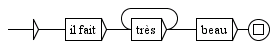
\includegraphics[width=7cm]{resources/img/fig10-1.png}
\caption{Graph with a cycle\label{cycle}}
\end{center}
\end{figure}

\end{itemize}







\section{Fst2Txt}\index{External programs!\verb+Fst2Txt+}\index{\verb+Fst2Txt+}
\label{section-Fst2Txt}
\verb+Fst2Txt [OPTIONS] <fst2>+

\bigskip
\noindent This program applies a transducer to a text in longest match mode at the
preprocessing stage, when the text has not been cut into lexical units yet.

\bigskip
\noindent \textbf{OPTIONS:}
\begin{itemize}
  \item \verb+-t TXT+/\verb+--text=TXT+: the text file to be
  modified, with extension \verb+.snt+;
  
  \item \verb+-a ALPH+/\verb+--alphabet=ALPH+: the alphabet file of the language of the
  text;\index{Alphabet}\index{File!alphabet}

  \item \verb+-s+/\verb+--start_on_space+: this parameter indicates that the
  search will start at any position in the text, even before a space. This 
  parameter should only be used to carry out morphological searches;
  
  \item \verb+-x+/\verb+--dont_start_on_space+: forbids the program to match
  expressions that start with a space (default);
  
  \item \verb+-c+/\verb+--char_by_char+: works in character by character
  tokenization mode. This is useful for languages like Thai;
  
  \item \verb+-w+/\verb+--word_by_word+: works in word by word
  tokenization mode (default);
\end{itemize}

\bigskip
\noindent \textbf{Output options:}
\begin{itemize}
  \item \verb+-M+/\verb+--merge+: merge transducer outputs with text inputs
  (default);
  \item \verb+-R+/\verb+--replace+: replace texts inputs with corresponding
  transducer outputs.
\end{itemize}

\bigskip
\noindent This program modifies the input text file.







\section{Grf2Fst2}\index{External programs!\verb+Grf2Fst2+}\index{\verb+Grf2Fst2+}
\index{Graph!compilation}\index{Compilation!of a graph}
\verb+Grf2Fst2 [OPTIONS] <grf>+

\bigskip
\noindent \index{File!\verb+.grf+}\index{File!\verb+.fst2+}
This program compiles a grammar into a \verb+.fst2+ file (for more details see
section \ref{section-graph-compilation}). The parameter \verb+<grf>+ 
denotes the complete path of the main graph of the grammar, without omitting the
extension \verb+.grf+.

\bigskip
\noindent \textbf{OPTIONS:}
\begin{itemize}
  \item \verb+-y+/\verb+--loop_check+: enables error checking (loop
  detection);
  \item \verb+-n+/\verb+--no_loop_check+: disables error checking (default);
  \index{Error detection in graphs}\index{Graph!error detection}\index{Errors in graphs}
  \item \verb+-a ALPH+/\verb+--alphabet=ALPH+: specifies the alphabet file to be
  used for tokenizing the content of the grammar boxes into lexical units;
  \item \verb+-c+/\verb+--char_by_char+: tokenization will be done character by
  character. If neither \verb+-c+ nor \verb+-a+ option is used, lexical units 
  will be sequences of any Unicode letters.
  \item \verb+-d DIR+/\verb+--pkgdir=DIR+: specifies the repository directory to
  use (see section \ref{section-repository}, page
  \pageref{section-repository}).
  \item \verb+-e+/\verb+--no_empty_graph_warning+: no warning will be emitted
  when a graph matches the empty word. This option is used by \verb+MultiFlex+
  in order not to scare users with meaningless error messages when they design
  an inflection grammar that matches the empty word. 
  \item \verb+-t+/\verb+--tfst_check+: checks wether the given graph can be
  considered as a valid sentence automaton or not.
  \item \verb+-s+/\verb+--silent_grf_name+: does not print the graph names
  (needed for consistent log files across several systems).
  \item \verb+-r XXX+/\verb+--named_repositories=XXX+: declaration of named
  repositories. XXX is made of one or more X=Y sequences, separated by `;', where
  X is the name of the repository denoted by pathname Y. You can use this 
  option several times.
  \item \verb+--debug+: compile graphs in debug mode.
  \item \verb+-v+/\verb+check_variables+: check output validity to avoid malformed variable expressions.
\end{itemize}

\bigskip
\noindent The result is a file with the same name as the graph passed to the
program as a parameter, but with extension \verb+.fst2+. This file is saved in
the same directory as \verb+<grf>+.


\section{GrfDiff}
		GrfDiff <grf1> <grf2>: .grf files to be compared

\noindent \textbf{OPTIONS:}
\begin{itemize}
  \item \verb+--output X+: saves the result, if any, in X instead of printing it on the output
\end{itemize}
         
         Compares the given grf files and prints their difference on the standard output. 
         Returns 0 if they are identical modulo box and transition reordering, 1 if there
		 are differences, 2 in case of error.
		 
		 Here are the diff indications that can be emitted:
\begin{itemize}
		 
		 \item \verb+P name+: a presentation property has changed. name=property name (SIZE, FONT, ...)
		 \item \verb+M a b+:  box moved. a=box number in <grf1>, b=box number in <grf2>
		 \item \verb+C a b+:  box content changed. a=box number in <grf1>, b=box number in <grf2>
		 \item \verb+A x+:    box added. x=box number in <grf2>
		 \item \verb+R x+:    box removed. x=box number in <grf1>
		 \item \verb+T a b x y+: transition added. a,b=src and dst box numbers in <grf1>. x,y=src and dst box numbers in <grf2>
		 \item \verb+X a b x y+: transition removed. a,b=src and dst box numbers in <grf1>. x,y=src and dst box numbers in <grf2>
\end{itemize}
		 
		 Note that transition modifications related to boxes that have been added or removed are not reported.





\section{GrfDiff3}
GrfDiff3 <mine> <base> <other>

  <mine>: my .grf file
  <other>: the other .grf file that may be conflicting
  <base>: the common ancestor .grf file

\bigskip
\noindent \textbf{OPTIONS:}
\begin{itemize}
\item \verb+--output+ \verb+X+: saves the result, if any, in X instead of printing it on the output
\item \verb+--conflicts+ \verb+X+: saves the description of the conflicts, if any, in X
\item \verb+--only-cosmetic+: reports a conflict for any change that is not purely cosmetic
\end{itemize}

Tries to merge <mine> and <other>. In case of success, the result is printed on the
standard output and 0 is returned. In case of unresolved conflicts, 1 is returned and
nothing is printed. 2 is returned in case of error.



\section{ImplodeTfst}
\index{External programs!\verb+ImplodeTfst+}
\index{\verb+ImplodeTfst+} \verb+ImplodeTfst [OPTIONS] <tfst>+

\bigskip
\noindent This program implodes the specified text automaton by merging
together lexical entries which only differ in their inflectional features.

\bigskip
\noindent \textbf{OPTIONS:}
\begin{itemize}
  \item \verb+-o OUT+/\verb+--output=OUT+: output file. By default, the input
  text automaton is modified.
\end{itemize}






\section{Locate}\index{External programs!\verb+Locate+}\index{\verb+Locate+}
\label{section-Locate}
\verb+Locate [OPTIONS] <fst2>+

\bigskip
\noindent \index{Pattern search}
This program applies a grammar to a text and constructs an index of the
occurrences found.

\bigskip
\noindent \textbf{OPTIONS:}
\begin{itemize}
  \item \verb+-t TXT+/\verb+--text=TXT+: complete path of the text file, without omitting
  the \verb+.snt+ extension;

  \item \verb+-a ALPH+/\verb+--alphabet=ALPH+: complete path of the alphabet
  file;\index{Alphabet}\index{File!alphabet}
  
  \item \verb+-m DICS+/\verb+--morpho=DICS+: this optional parameter indicates
  which morphological-mode dictionaries are to be used, if needed by some \verb+.fst2+
  dictionaries. \verb+DICS+ represents a list of \verb+.bin+ files (with full
  paths) separated with semi-colons;
  
  \item \verb+-s+/\verb+--start_on_space+: this parameter indicates that the
  search will start at any position in the text, even before a space. This 
  parameter should only be used to carry out morphological searches;
  
  \item \verb+-x+/\verb+--dont_start_on_space+: forbids the program to match
  expressions that start with a space (default);
  
  \item \verb+-c+/\verb+--char_by_char+: works in character by character
  tokenization mode. This is useful for languages like Thai;
  
  \item \verb+-w+/\verb+--word_by_word+: works in word by word
  tokenization mode (default);
  
  \item \verb+-d DIR+/\verb+--sntdir=DIR+: puts produced files in \verb+DIR+
  instead of the text directory. Note that \verb+DIR+ must end with a file separator
  (\verb+\+ or \verb+/+);
  
  \item \verb+-K+/\verb+--korean+: tells \verb+Locate+ that it works on Korean;

  \item \verb+-u X+/\verb+--arabic_rules=X+: Arabic typographic rule configuration file;

  \item \verb+-g X+/\verb+--negation_operator=X+: specifies the negation operator to be used in
  Locate patterns. The two legal values for \verb+X+ are \verb+minus+ and \verb+tilde+ (default).
  Using \verb+minus+ provides backward compatibility with previous versions of Unitex.
\end{itemize}

\bigskip
\noindent \textbf{Search limit options:}
\begin{itemize}
  \item \verb+-l+/\verb+--all+: looks for all matches (default);
  \item \verb+-n N+/\verb+--number_of_matches=N+: stops after the first
  \verb+N+ matches.
\end{itemize}

\bigskip
\noindent \textbf{Maximum iterations per token options:}
\begin{itemize}
  \item \verb+-o N+/\verb+--stop_token_count=N+: stops after N iterations on a token;
  \item \verb+-o N,M+/\verb+--stop_token_count=N,M+: emits a warning after N iterations on a token and stops after M iterations.
\end{itemize}

\bigskip
\noindent \textbf{Matching mode options:}
\begin{itemize}
  \item \verb+-S+/\verb+--shortest_matches+;
  \item \verb+-L+/\verb+--longest_matches+ (default);
  \item \verb+-A+/\verb+--all_matches+.
\end{itemize}

\bigskip
\noindent \textbf{Output options:}
\begin{itemize}
  \item \verb+-I+/\verb+--ignore+: ignore transducer outputs (default);
  \item \verb+-M+/\verb+--merge+: merge transducer outputs with text inputs;
  \item \verb+-R+/\verb+--replace+: replace texts inputs with corresponding
  transducer outputs;
  \item \verb+-p+/\verb+--protect_dic_chars+: when \verb+-M+ or \verb+-R+ mode is
  used, \verb+-p+ protects some input characters with a backslash. This is useful
  when \verb+Locate+ is called by \verb+Dico+ in order to avoid producing bad
  lines like:
  
  %do not remove this line jump
  \verb+3,14,.PI.NUM+
  \item \verb+-v X=Y+/\verb+--variable=X=Y+: sets an output variable named X with content Y. 
  Note that Y must be ASCII.
\end{itemize}

\bigskip
\noindent \textbf{Ambiguous output options:}
\begin{itemize}
  \item \verb+-b+/\verb+--ambiguous_outputs+: allows the production of several 
  matches with same input but different outputs (default);
  \item \verb+-z+/\verb+--no_ambiguous_outputs+: forbids ambiguous outputs. In
  case of ambiguous outputs, one will be arbitrarily chosen and kept, depending on the
  internal state of the program.
\end{itemize}

\bigskip
\noindent \textbf{Variable error options}

\noindent These options have no effect if the output mode is set with
\verb+--ignore+; otherwise, they rule the behavior of the \verb+Locate+ program
when an output is found that contains a reference to a variable that is not correctly defined.
\begin{itemize}
  \item \verb+-X+/\verb+--exit_on_variable_error+: kills the program;
  \item \verb+-Y+/\verb+--ignore_variable_errors+: acts as if the variable has
  an empty content (default);
  \item \verb+-Z+/\verb+--backtrack_on_variable_errors+: stop exploring the
  current path of the grammar.
\end{itemize}
  
\bigskip
\noindent \textbf{Variable injection:}
\begin{itemize}
	\item \verb+-v X=Y+/\verb+--variable=X=Y+: sets an output variable named X with content Y. 
	Note that Y must be ASCII
\end{itemize}

\bigskip
\noindent \index{File!\verb+concord.ind+}\index{File!\verb+concord.n+}This 
program saves the references to the found occurrences in a file called
\verb+concord.ind+. The number of occurrences, the number of units belonging to
those occurrences, as well as the percentage of recognized units within the text
are saved in a file called \verb+concord.n+. These two files are stored in the
directory of the text.







\section{LocateTfst}\index{External programs!\verb+LocateTfst+}\index{\verb+LocateTfst+}
\label{section-LocateTfst}
\verb+LocateTfst [OPTIONS] <fst2>+

\bigskip
\noindent \index{Pattern search}
Applies a grammar to a text automaton, and saves the matching sequence index in a
file named \verb+concord.ind+, just as \verb+Locate+ does.

\bigskip
\noindent \textbf{OPTIONS:}
\begin{itemize}
  \item \verb+-t TFST+/\verb+--text=TFST+: complete path of the text automaton,
  without omitting the \verb+.tfst+ extension;

  \item \verb+-a ALPH+/\verb+--alphabet=ALPH+: complete path of the alphabet
  file;\index{Alphabet}\index{File!alphabet}
  
  \item \verb+-K+/\verb+--korean+: tells \verb+LocateTfst+ that it works on
  Korean;

  \item \verb+-g X+/\verb+--negation_operator=X+: specifies the negation operator to be used in
  Locate patterns. The two legal values for \verb+X+ are \verb+minus+ and \verb+tilde+ (default).
  Using \verb+minus+ provides backward compatibility with previous versions of Unitex.
  
\end{itemize}

\bigskip
\noindent \textbf{Search limit options:}
\begin{itemize}
  \item \verb+-l+/\verb+--all+: looks for all matches (default);
  \item \verb+-n N+/\verb+--number_of_matches=N+: stops after the first
  \verb+N+ matches.
\end{itemize}

\bigskip
\noindent \textbf{Matching mode options:}
\begin{itemize}
  \item \verb+-S+/\verb+--shortest_matches+;
  \item \verb+-L+/\verb+--longest_matches+ (default);
  \item \verb+-A+/\verb+--all_matches+.
\end{itemize}

\bigskip
\noindent \textbf{Output options:}
\begin{itemize}
  \item \verb+-I+/\verb+--ignore+: ignore transducer outputs (default);
  \item \verb+-M+/\verb+--merge+: merge transducer outputs with text inputs;
  \item \verb+-R+/\verb+--replace+: replace texts inputs with corresponding
  transducer outputs.
\end{itemize}

\bigskip
\noindent \textbf{Ambiguous output options:}
\begin{itemize}
  \item \verb+-b+/\verb+--ambiguous_outputs+: allows the production of several 
  matches with same input but different outputs (default);
  \item \verb+-z+/\verb+--no_ambiguous_outputs+: forbids ambiguous outputs. In
  case of ambiguous outputs, one will be arbitrarily chosen and kept, depending on the
  internal state of the program.
\end{itemize}

\bigskip
\noindent \textbf{Variable error options}

\noindent These options have no effect if the output mode is set with
\verb+--ignore+; otherwise, they rule the behavior of the \verb+Locate+ program
when an output is found that contains a reference to a variable that is not correctly defined.
\begin{itemize}
  \item \verb+-X+/\verb+--exit_on_variable_error+: kills the program;
  \item \verb+-Y+/\verb+--ignore_variable_errors+: acts as if the variable has
  an empty content (default);
  \item \verb+-Z+/\verb+--backtrack_on_variable_errors+: stop exploring the
  current path of the grammar.
\end{itemize}
\noindent \textbf{Variable injection}
\begin{itemize}
  \item \verb+-v X=Y+/\verb+--variable=X=Y+: sets an output variable named X with content Y. 
  Note that Y must be ASCII.
\end{itemize}
\noindent \textbf{Tagging option}
\begin{itemize}
  \item \verb+--tagging+: indicates that the concordance must be a tagging one, containing
  additional information on the start and end states of each match.
\end{itemize}
\bigskip
\noindent \index{File!\verb+concord.ind+}\index{File!\verb+concord_tfst.n+}This 
program saves the references to the found occurrences in a file called
\verb+concord.ind+. The number of occurrences and the number of produced outputs
are saved in a file called \verb+concord_tfst.n+. These two files are stored in the
directory of the text.







\section{MultiFlex}\index{External programs!\verb+MultiFlex+}\index{\verb+MultiFlex+}
\verb+MultiFlex [OPTIONS] <dela>+

\bigskip
\noindent \index{Dictionaries!automatic inflection}\index{Automatic inflection}This 
program carries out the automatic inflection of a DELA dictionary 
containing simple (see section \ref{section-DELAS-format}) or compound word
lemmas (see chapter \ref{chap-multiflex}).

\bigskip
\noindent \textbf{OPTIONS:}
\begin{itemize}
  \item \verb+-o DELAF+/\verb+--output=DELAF+: output DELAF file;
  \item \verb+-a ALPH+/\verb+--alphabet=ALPH+: alphabet file;
  \item \verb+-d DIR+/\verb+--directory=DIR+: the directory containing
  \verb+Morphology+ and \verb+Equivalences+ files and inflection graphs for
                                              single and compound words;
  \item \verb+-K+/\verb+--korean+: tells \verb+MultiFlex+ that it works on
  Korean;
  \item \verb+-s+/\verb+--only-simple-words+: the program will consider
  compound words as errors;
  \item \verb+-c+/\verb+--only-compound-words+: the program will consider
  simple words as errors;
  \item \verb+-p DIR+/\verb+--pkgdir=DIR+: specifies the graph repository.
  \item \verb+-rXXX+/\verb+--named_repositories=XXX+: declaration of named
  repositories. XXX is made of one or more X=Y sequences, separated by ; 
  where X is the name of the repository denoted by the pathname Y. You 
  can use this option several times.
  
\end{itemize}\index{Hangul}\index{Hangul}

\bigskip
\noindent Note that \verb+.fst2+ inflection transducers will automatically be
built from corresponding \verb+.grf+ files if absent or older than \verb+.grf+
files.







\section{Normalize}\index{External programs!\verb+Normalize+}\index{\verb+Normalize+}
\label{section-Normalize}
\index{Text!normalization}
\verb+Normalize [OPTIONS] <text>+

\bigskip
\noindent \index{Normalization!of separators}This 
program carries out a normalization of text separators. The separators are
space, tab, and newline. Every sequence of separators that contains at least one
newline is replaced by a unique newline. All other sequences of separators are
replaced by a single space.

\bigskip
\noindent This program also checks the syntax of lexical tags found in the text. All
sequences in curly brackets should be either the sentence delimiter \verb+{S}+,
the stop marker \verb+{STOP}+, or valid entries in the DELAF format (\verb+{aujourd'hui,.ADV}+). 
\index{\verb+{S}+}\index{Sentence delimiter}

\bigskip
\noindent \index{Lexical!labels}Parameter \verb+<text>+ 
represents the complete path of the text file. The program
creates a modified version of the text that is saved in a file with extension
\verb+.snt+.\index{File!\verb+.snt+}

\bigskip
\noindent \textbf{OPTIONS:}
\begin{itemize}
  \item \verb+-n+/\verb+--no_carriage_return+: every separator sequence will be turned into a single space;
  \item \verb+--input_offsets=XXX+: base offset file to be used.
  \item \verb+--output_offsets=XXX+: offset file to be produced.
  \item \verb+-r XXX+/\verb+--replacement_rules=XXX+: specifies the
  normalization rule file to be used. See section \ref{section-normalization-file} 
  for details about the format of
  this file. By default, the program only replaces \verb+{+ and \verb+}+ by
  \verb+[+ and \verb+]+.
  \item \verb+--no_separator_normalization+: only applies replacement rules specified with -r
\end{itemize}

\bigskip
\noindent WARNING: if you specify a normalization rule file, its rules will be
applied prior to anything else. So, you have to be very careful if you
manipulate separators in such rules.






\section{PolyLex}\index{External programs!\verb+PolyLex+}\index{\verb+PolyLex+}
\verb+PolyLex [OPTIONS] <list>+
\index{Norwegian!free compound words}\index{German!free compound words}\index{Dutch!free compound words}
\index{Russian!free compound words}
\index{Analysis of free compound words!in Germanic languages}\index{Words!compound!in Germanic languages}
\index{Analysis of free compound words!in Russian}\index{Words!compound!in Russian}

\bigskip
\noindent This program takes a file containing unknown words \verb+<list>+ and
tries to analyse each of the words as a compound obtained by concatenating simple words. The words
that have at least one analysis are removed from the file of unknown words and
the dictionary lines that correspond to the analysis are appended to file
\verb+OUT+. 

\bigskip
\noindent \textbf{OPTIONS:}
\begin{itemize}
  \item \verb+-a ALPH+/\verb+--alphabet=ALPH+: the alphabet file to use;

  \item \verb+-d BIN+/\verb+--dictionary=BIN+: .bin dictionary to use;

  \item \verb+-o OUT+/\verb+--output=OUT+: designates the file in which the 
  produced dictionary lines are to be printed; if that file already exists, 
  the produced lines are appended at the end of the file;

  \item \verb+-i INFO+/\verb+--info=INFO+: designates a text file in which 
  the information about the analysis has been produced.
\end{itemize}

\bigskip
\noindent \textbf{Language options:}
\begin{itemize}
  \item \verb+-D+/\verb+--dutch+
  \item \verb+-G+/\verb+--german+
  \item \verb+-N+/\verb+--norwegian+
  \item \verb+-R+/\verb+--russian+
\end{itemize}  

\bigskip
\noindent NOTE: for Dutch or Norwegian words, the program tries to read a text
file containing a list of forbidden words. This file is supposed to be named
\verb+ForbiddenWords.txt+ (see section \ref{section-forbidden-words}) and stored
in the same directory than \verb+BIN+.






\section{RebuildTfst}\index{External
programs!\verb+RebuildTfst+}\index{\verb+RebuildTfst+}
\verb+RebuildTfst <tfst>+

\bigskip
\noindent \index{Text!automaton of the}\index{Reconstruction of the text automaton}This 
program reconstructs text automaton \verb+<tfst>+ taking into account the
manual modifications. If the program finds a file \verb+sentenceN.grf+ in the
same directory as \verb+<tfst>+, it replaces the automaton of sentence
\verb+N+ with the one represented by \verb+sentenceN.grf+. The input text
automaton is modified.






\section{Reconstrucao}\index{External programs!\verb+Reconstrucao+}\index{\verb+Reconstrucao+}
\index{Compression of a dictionary}\index{Dictionaries!compression}
\index{Clitics!normalization}\index{Normalization!of clitics in Portuguese}
\index{Portuguese!normalization of clitics}
\verb+Reconstrucao [OPTIONS] <index>+

\bigskip
\noindent This program generates a normalization grammar designed to be applied
before the construction of an automaton for a Portuguese text. The \verb+<index>+ file
represents a concordance which has to be produced by applying in MERGE mode to
the considered text a grammar that extracts all forms to be normalized. This
grammar is called \verb+V-Pro-Suf+, and is stored in the
\verb+/Portuguese/Graphs/Normalization+ directory.

\bigskip
\noindent \textbf{OPTIONS:}
\begin{itemize}
  \item \verb+-a ALPH+/\verb+--alphabet=ALPH+: the alphabet file to use;

  \item \verb+-r ROOT+/\verb+--root=ROOT+: the inverse \verb+.bin+
  dictionary to use to find forms in the future and conditional given their
  canonical forms. It has to be obtained by compressing the dictionary of verbs
  in the future and conditional with the parameter \verb+--flip+ (see section
  \ref{section-compress});
  
  \item \verb+-d BIN+/\verb+--dictionary=BIN+: the \verb+.bin+ dictionary to use;
  
  \item \verb+-p PRO+/\verb+--pronoun_rules=PRO+: the \verb+.fst2+ grammar
  describing pronoun rewriting rules;
  
  \item \verb+-n PRO+/\verb+--nasal_pronoun_rules=PRO+: the \verb+.fst2+ grammar
  describing nasal pronoun rewriting rules;

  \item \verb+-o OUT+/\verb+--output=OUT+: the name of the \verb+.grf+ graph to
  be generated.
\end{itemize}







\section{Reg2Grf}\index{External programs!\verb+Reg2Grf+}\index{\verb+Reg2Grf+}
\verb+Reg2Grf <txt>+

\bigskip
\noindent \index{Regular expressions}\index{File!\verb+.grf+}\index{File!\verb+regexp.grf+}This 
program constructs a \verb+.grf+ file corresponding to the regular
expression written in file \verb+<txt>+. The parameter \verb+<txt>+ represents the
complete path to the file containing the regular expression. This file needs to
be a Unicode text file. The program takes into account all characters up to the
first newline. The result file is called \verb+regexp.grf+ and is saved in the
same directory as \verb+<txt>+.





\section{Seq2Grf}\index{External programs!\verb+Seq2Grf+}
\index{\verb+Seq2Grf+}
\label{Seq2Grf}
\verb+Seq2Grf [OPTIONS] <snt>+

\index{Sorting}
\bigskip
\noindent This program constructs a \verb+.grf+ file 
corresponding to the sequences contained in file \verb+<snt>+. 

\bigskip
\noindent \textbf{OPTIONS:}

\begin{itemize}
  \item \verb+-a ALPH+/\verb+--alphabet=ALPH+: the alphabet file to use;
  \item \verb+-o XXX+/\verb+--output=XXX+: output GRF file;
  \item \verb+-s+/\verb+--only-stop+: only consider {STOP}-separated sequences;
  \item \verb+-b+/\verb+--beautify+: apply the grf beautifying algorithm;
  \item \verb+-n+/\verb+--no_beautify+: do not apply the grf beautifying algorithm (default);
  \item \verb+--case-sensitive+: all letter tokens are protected with double-quotes (default);
  \item \verb+--case-insensitive+: letter tokens are not protected with double-quotes;
  \item \verb+-w x+: number of wildcards;
  \item \verb+-i x+: number of insertions;
  \item \verb+-r x+: number of replations;
  \item \verb+-d x+: number of deletions;
\end{itemize}

\bigskip
\noindent Constructs the sequences automaton : one single automaton that recognizes
	all the sequences from the SNT.
	The sequences must be delimited with the special tag \{STOP\}.
	The produced .grf file is stored in the user's Graphs directory
	The other files, named \verb+text.tfst+, \verb+text.tind+ are stored in the text directory.

\section{SortTxt}\index{External programs!\verb+SortTxt+}\index{\verb+SortTxt+}

\verb+SortTxt [OPTIONS] <txt>+

\index{Sorting}
\bigskip
\noindent This program carries out a lexicographical sorting of the lines of file
\verb+<txt>+. \verb+<txt>+ represents the complete path of the file to be sorted.

\bigskip
\noindent \textbf{OPTIONS:}
\begin{itemize}
  \item \verb+-n+/\verb+--no_duplicates+: remove duplicate lines (default);

  \item \verb+-d+/\verb+--duplicates+: remove duplicate lines;

  \item \verb+-r+/\verb+--reverse+: sort in descending order;

  \item \verb+-o XXX+/\verb+--sort_order=XXX+: sorts using the alphabet of the
  order defined by file \verb+XXX+. If this parameter is missing, the sorting is done according to the
  order of Unicode characters;

  \item \verb+-l XXX+/\verb+--line_info=XXX+: backup the number of lines of the result file in
  file \verb+XXX+;
  
  \item \verb+-t+/\verb+--thai+: option for sorting Thai text.
  \item \verb+-f+/\verb+--factorize_inflectional_codes+: makes two entries XXX,YYY.ZZZ:A and XXX,YYY.ZZZ:B
                                   become a single entry XXX,YYY.ZZZ:A:B
\end{itemize}

\bigskip
\noindent The input text file is modified. By default,
the sorting is performed in the order of Unicode characters, removing duplicate lines.








\section{Stats}\index{External programs!\verb+Stats+}\index{\verb+Stats+}

\verb+Stats [OPTIONS] <ind>+

\index{Statistics}
\bigskip
\noindent This program computes some statistics from the \verb+<ind>+
concordance index file.

\bigskip
\noindent \textbf{OPTIONS:}
\begin{itemize}
  \item \verb+-m MODE+/\verb+--mode=MODE+: specifies the output to be produced:
  \begin{itemize}
      \item \verb+0+ = matches with left and right contexts + number of
      occurrences;
      \item \verb+1+ = collocates + number of occurrences;
      \item \verb+2+ = collocates + number of occurrences + z-score.
  \end{itemize}

  \item \verb+-a ALPH+/\verb+--alphabet=ALPH+: alphabet file to use;

  \item \verb+-o OUT+/\verb+--output=OUT+: output file;

  \item \verb+-l N+/\verb+--left=N+: length of left contexts in tokens;
   
  \item \verb+-r N+/\verb+--right=N+: length of right contexts in tokens;
  
  \item \verb+-c N+/\verb+--case=N+: case policy: \verb+0+ = case insensitive,
  \verb+1+ = case sensitive (default).
\end{itemize}







\section{Table2Grf}\index{External programs!\verb+Table2Grf+}\index{\verb+Table2Grf+}
\verb+Table2Grf [OPTIONS] <table>+

\bigskip
\noindent \index{Lexicon-grammar!tables}\index{Graph!main}This 
program automatically generates graphs from a lexicon-grammar \verb+<table>+
and a template graph.

\bigskip
\noindent \textbf{OPTIONS:}
\begin{itemize}
  \item \verb+-r GRF+/\verb+--reference_graph=GRF+: name of the template graph;
  
  \item \verb+-o OUT+/\verb+--output=OUT+: name of the result main graph;
  
  \item \verb+-s XXX+/\verb+--subgraph_pattern=XXX+: if this optional parameter
  if specified, all the produced subgraphs will be named according to this pattern. 
  In order to have unambiguous names, we recommend to include \verb+@%+ in the parameter 
  (remind that \verb+@%+ will be replaced by the line number of the entry in the table). 
  For instance, if you set the pattern parameter to '\verb+subgraph-@%.grf+', 
  subgraph names will be such as '\verb+subgraph-0013.grf+'. By default,
  subgraph names look like '\verb+result_0013.grf+', where '\verb+result.grf+' 
  designates the result main graph.
\end{itemize}






\section{Tagger}\index{External programs!\verb+Tagger+}\index{\verb+Tagger+}
\verb+Tagger [OPTIONS] <tfst>+
\label{section-Tagger}

\bigskip
\noindent The input of this program is the text automaton in the specified \verb+.tfst+. The program applies
the Viterbi-Path algorithm to it and produces a linear automaton. The automaton is pruned in a probabilistic way based on
a second-order hidden Markov model. If the specified tagger data file contains tuples of "cat" tags,
the tagger prunes transitions on the basis of grammatical, syntactic and semantic codes (for example, \verb$that.DET+Ddem$ versus 
\verb$that.PRO+Pdem$). Else if it contains tuples of "morph" tags, so the tagger prunes transitions on grammatical, semantic,
syntactic and inflectional codes (\verb$the.DET+Ddef:s$ versus \verb$the.DET+Ddef:p$). In that case, the automaton needs to be 
exploded before applying the tagging process and a tagset file must be specified by the \verb+-t+ option below.

\bigskip
\noindent \textbf{OPTIONS:}
\begin{itemize}
  \item \verb+-a ALPH+/\verb+--alphabet=ALPH+: alphabet file.
  \item \verb+-o OUT+/\verb+--output=OUT+: output text automaton.
  \item \verb+-t TAGSET+/\verb+--tagset=TAGSET+: name of the tagset description file.
  \item \verb+-d DATA+/\verb+--data=DATA+: a .bin tagger data file that contains occurrence counts 
  for unigrams, bigrams and trigrams in order to compute probabilities. This file is obtained with 
  the \verb+TrainingTagger+ program (see section \ref{section-training-dict}).
\end{itemize}





\section{TagsetNormTfst}\index{External
programs!\verb+TagsetNormTfst+}\index{\verb+TagsetNormTfst+} \verb+TagsetNormTfst [OPTIONS] <tfst>+

\bigskip
\noindent This program normalizes the specified \verb+.tfst+ text automaton according
to a tagset description file, discarding undeclared dictionary codes
and incoherent lexical entries. Inflectional features are unfactorized so 
that \verb+{rouge,.A:fs:ms}+ will be divided into the 2 tags \verb+{rouge,.A:fs}+ 
and \verb+{rouge,.A:ms}+.

\bigskip
\noindent \textbf{OPTIONS:}
\begin{itemize}
  \item \verb+-o OUT+/\verb+--output=OUT+: output text automaton. By default,
  the input text automaton is modified;
  \item \verb+-t TAGSET+/\verb+--tagset=TAGSET+: name of the tagset description
  file.
\end{itemize}







\section{TEI2Txt}\index{External programs!\verb+TEI2Txt+} 
\index{\verb+TEI2Txt+}
\verb+TEI2Txt [OPTIONS] <xml>+

\bigskip
\noindent Produces a raw text file from the given \verb+<xml>+ TEI file.

\bigskip
\noindent \textbf{OPTIONS:}
\begin{itemize}
  \item \verb+-o TXT+/\verb+--output=TXT+: name of the output text file.
  By default, the output file has the same name than the input one, 
  replacing \verb+.xml+ by \verb+.txt+.
\end{itemize}







\section{Tfst2Grf}\index{External
programs!\verb+Tfst2Grf+}\index{\verb+Tfst2Grf+}
\index{Automaton!of the text}\index{Text!automaton of the}
\verb+Tfst2Grf [OPTIONS] <tfst>+

\bigskip
\noindent This program extracts a sentence automaton in \verb+.grf+ format from
the given text automaton. 

\bigskip
\noindent \textbf{OPTIONS:}
\begin{itemize}
  \item \verb+-s N+/\verb+--sentence=N+: the number of the sentence to be
  extracted;
  
  \item \verb+-o XXX+/\verb+--output=XXX+: pattern used to name output files 
 \verb+XXX.grf+, \verb+XXX.txt+ and \verb+XXX.tok+ (default=\verb+cursentence+);
 
  \item \verb+-f FONT+/\verb+--font=FONT+: sets the font to be used in the
  output \verb+.grf+
   
%DO NOT REMOVE THIS LINE JUMP
  (default=\verb+Times new Roman+);
  \item \verb+-z N+/\verb+--fontsize=N+: sets the font size (default=10).
\end{itemize}

\bigskip
\noindent The program produces the following files and saves them in the
directory of the text:

\begin{itemize}
  \item \verb+cursentence.grf+: graph representing the automaton of the
  sentence;\index{File!\verb+cursentence.grf+}

  \item \verb+cursentence.txt+: text file containing the
  sentence;\index{File!\verb+cursentence.txt+}

  \item \verb+cursentence.tok+: text file containing the
  numbers of the tokens that compose the
  sentence.\index{File!\verb+cursentence.tok+}
\end{itemize}







\section{Tfst2Unambig}\index{External
programs!\verb+Tfst2Unambig+}\index{\verb+Tfst2Unambig+}
\index{Text!automaton of the!conversion into linear text}
\verb+Tfst2Unambig [OPTIONS] <tfst>+

\bigskip
\noindent This programs takes a \verb$.tfst$ text automaton and produces an
equivalent text file if the automaton is linear (i.e. with no
ambiguity). See section \ref{section-linear-text}, page \pageref{section-linear-text}.

\bigskip
\noindent \textbf{OPTIONS:}
\begin{itemize}
  \item \verb+-o TXT+/\verb+--out=TXT+: the output text file.
\end{itemize}







\section{Tokenize}\index{External programs!\verb+Tokenize+}\index{\verb+Tokenize+}
\label{section-Tokenize}
\index{Text!tokenization}\index{Tokenization}\index{Token}
\verb+Tokenize [OPTIONS] <txt>+

\index{Lexical!unit}\index{File!\verb+.snt+}\index{Alphabet}\index{File!alphabet} 
\bigskip
\noindent This program tokenizes a tet text into lexical units.
\verb+<txt>+ the complete path of the text file, without omitting the \verb+.snt+ 
extension.

\bigskip
\noindent \textbf{OPTIONS:}
\begin{itemize}
  \item \verb+-a ALPH+/\verb+--alphabet=ALPH+: alphabet file;
  
  \item \verb+-c+/\verb+--char_by_char+: indicates whether the program is applied character by
  character, with the exceptions of the sentence delimiter \verb+{S}+,
  the stop marker \verb+{STOP}+ and lexical tags like \verb+{today,.ADV}+ which
  are considered to be single units;

 \item \verb+-w+/\verb+--word_by_word+: with this option, the program
  considers a unit to be either a sequence of letters (the letters are defined
  by file \verb+alphabet+), or a character which is not a letter, or the
  sentence separator \verb+{S}+\index{\verb+{S}+}, or a lexical label 
  like \verb+{aujourd'hui,.ADV}+. \index{Sentence delimiter}
  \index{Lexical!labels} This is the default mode.

 \item \verb+-t TOKENS+/\verb+--tokens=TOKENS+: specifies a \verb+tokens.txt+
 file to load and modify, instead of creating a new one from scratch.
\end{itemize}
\bigskip
\noindent \textbf{Offsets options:}
\begin{itemize}
  \item \verb+input_offsets+: base offset file to be used;
  \item \verb+output_offsets+: offset file to be produced;
\end{itemize}


\index{File!\verb+tokens.txt+}\index{File!\verb+text.cod+}
\bigskip
\noindent The program codes each unit as a whole. The list of units is saved in a text file
called \verb+tokens.txt+. The sequence of codes representing the units now allows
the coding of the text. This sequence is saved in a binary file named
\verb+text.cod+. The program also produces the following four files:

\begin{itemize}
  \item \verb+tok_by_freq.txt+: text file containing the units sorted by frequency;
  \item \verb+tok_by_alph.txt+: text file containing the units sorted alphabetically;
  \item \verb+stats.n+: text file containing information on the number of
  sentence separators, the number of units, the number of simple words and the
  number of numbers;

  \item \verb+enter.pos+: binary file containing the list of newline positions in
  the text. The coded representation of the text does not contain newlines, but
  spaces. Since a newline counts as two characters and a space as a single one,
  it is necessary to know where newlines occur in the text when the positions of
  occurrences located by the \verb+Locate+ program are to be synchronized with
  the text file. File \verb+enter.pos+ is used for this by the \verb+Concord+
  program. Thanks to this, when clicking on an occurrence in a concordance, it is
  correctly selected in the text. File \verb$enter.pos$ is a binary file
  containing the list of the positions of newlines in the text.

\end{itemize}
\index{File!\verb+tok_by_freq.txt+}\index{File!\verb+tok_by_alph.txt+}
\index{File!\verb+stats.n+}\index{File!\verb+enter.pos+}

\bigskip
\noindent All produced files are saved in the text directory.






\section{TrainingTagger}\index{External programs!\verb+TrainingTagger+}\index{\verb+TrainingTagger+}
\verb+TrainingTagger [OPTIONS] <txt>+
\label{section-TrainingTagger}

\bigskip
\noindent \index{Lexicon-grammar!tables}\index{Graph!main}This 
program automatically generates two tagger data files from a tagged corpus text file. They are used by the \verb+Tagger+ program 
in order to compute probabilities and linearize the text automaton. The tagged corpus file must follow the format described 
in section \ref{section-corpus-file}. Those files contain tuples (unigrams, bigrams and trigrams), 
formed by tags and words. In the first data file, tags are "cat" tags (i.e. grammatical, syntactic and semantic codes). 
In the second data file, tags are "morph" tags (i.e. grammatical, syntactic, semantic and inflectional codes). 

\bigskip
\noindent \textbf{OPTIONS:}
\begin{itemize}
  \item \verb+-a/--all+: indicates whether the program should produce all data files (default);
  \item \verb+-c/--cat+: indicates whether the program should produce only data file with "cat" tags;
  \item \verb+-m/--morph+: indicates whether the program should produce only data file with "morph" tags;
  \item \verb+-n/--no_binaries+: indicates whether the program should not compress data files into
  \verb+.bin+ files, in this case only \verb+.dic+ data files are generated;
  \item \verb+-b/--binaries+: indicates whether the program should compress data files into 
  \verb+.bin+ files (default);
  \item \verb+-o XXX/--output=XXX+: pattern used to name output tagger data files \verb+XXX_data_cat.bin+
  and \verb+XXX_data_morph.bin+ (default=filename of text corpus without extension);
  \item \verb+-s/--semitic+: indicates that the semitic compression algorithm should be used.
\end{itemize}

\bigskip

\section{Txt2Tfst}\index{External
programs!\verb+Txt2Tfst+}\index{\verb+Txt2Tfst+} \verb+Txt2Tfst [OPTIONS] <txt>+

\index{Automaton!of the text}\index{Text!automaton of the}\index{File!\verb+.snt+}
\index{File!alphabet}\index{Alphabet}
\bigskip
\noindent This program constructs an automaton of a text. \verb+<txt>+
represents the complete path of a text file without omitting the \verb+.snt+
extension.

\bigskip
\noindent \textbf{OPTIONS:}
\begin{itemize}
  \item \verb+-a ALPH+/\verb+--alphabet=ALPH+: alphabet file;
  
  \item \verb+-c+/\verb+--clean+: indicates whether the rule of conservation of 
  the best paths (see section \ref{section-keeping-best-paths}) 
  should be applied\index{Conservation of better paths};
  
  \item \verb+-n XXX+/\verb+--normalization_grammar=XXX+: name of a normalization 
  grammar that is to be applied to the text automaton; \index{Normalization!of ambiguous forms}
  \index{Normalization!of the text automaton}
  \item \verb+-t TAGSET+/\verb+--tagset=TAGSET+: Elag tagset file to use to
  normalize dictionary entries;
  \item \verb+-K+/\verb+--korean+: tells \verb+Txt2Tfst+ that it works on
  Korean.
\end{itemize}

\bigskip
\noindent If the text is separated into sentences, the program constructs an
automaton for each sentence. If this is not the case, the program arbitrarily
cuts the text into sequences of 2000 tokens and produces an automaton for
each of these sequences.\index{Lexical!unit}\index{Token}

\index{File!\verb+text.tfst+}\index{File!\verb+text.tind+}
\bigskip
\noindent The result is a file called \verb+text.tfst+ which is saved in the directory of
the text. Another file named \verb+text.tind+ is also produced.

\bigskip
\noindent NOTE: The program will also try to use the \verb+tags.ind+ file, if
any (see section \ref{section-tags-ind}).







\section{Uncompress}\index{External
programs!\verb+Uncompress+}\index{\verb+Uncompress+}
\label{section-Uncompress}
\verb+Uncompress [OPTIONS] <bin>+

\bigskip
\noindent This program uncompresses a \verb+.bin+ dictionary into a text file
\verb+.dic+ one.

\bigskip
\noindent \textbf{OPTIONS:}
\begin{itemize}
  \item \verb+-o OUT+/\verb+--output=OUT+: optional output file name (default:
  \verb+file.bin+ > \verb+file.dic+).
\end{itemize}








\section{Untokenize}\index{External
programs!\verb+Untokenize+}\index{\verb+Untokenize+}
\label{section-Untokenize}
\verb+Untokenize [OPTIONS] <txt>+

\bigskip
\noindent Untokenizes and rebuild the orgininal text. The token list is stored into \verb+tokens.txt+ and
         the coded text is stored into \verb+text.cod+.
         The file \verb+enter.pos+ contains the position in tokens of all the carriage return sequences.
         These files are located in the XXX\_snt directory where XXX is <txt> without its extension.

\bigskip
\noindent \textbf{OPTIONS:}
\begin{itemize}

  \item \verb+-d X+/\verb+--sntdir=X+: uses directory X instead of the text directory; note that X must be (back)slash terminated
  \item \verb+-n N+/\verb+--number_token=N+: adds tokens number each N token;
  \item \verb+-r N+/\verb+--range=N+: emits only token from number N to end;
  \item \verb+-r N,M+/\verb+--range=N,M+: emits only token from number N to M.
\end{itemize}








\section{UnitexTool}\index{External
programs!\verb+UnitexTool+}\index{\verb+UnitexTool+}\index{Scripting Unitex programs}
\label{section-UnitexTool}
\verb+UnitexTool <utilities>+

\bigskip
\noindent This program is a super-program that allows you to invoke all Unitex
external programs. With it, you can chain commands so that they will be invoked
within a same system process, in order to speed up processing. This can done by
invoking commands nested in round brackets as this:

\bigskip
\begin{verbatim}
UnitexTool { SelectOutput [OPTIONS] } 
             { cmd #1+args } 
             { cmd #2+args }
             etc.
\end{verbatim}

\bigskip
\noindent For instance, if you want to join a locate operation and the
construction of the concordance, you can use the following command:

\bigskip
\begin{verbatim}
UnitexTool { Locate "-tD:\My Unitex\English\Corpus\ivanhoe.snt" 
"D:\My Unitex\English\regexp.fst2"
"-aD:\My Unitex\English\Alphabet.txt" -L -I -n200 
"--morpho=D:\Unitex2.0\English\Dela\dela-en-public.bin" -b -Y }
{ Concord "D:\My Unitex\English\Corpus\ivanhoe_snt\concord.ind" 
"-fCourier new" -s12 -l40 -r55 --CL --html 
"-aD:\My Unitex\English\Alphabet_sort.txt" }
\end{verbatim}

\bigskip
\noindent \textbf{OPTIONS}:
\begin{itemize}
\item \verb+-o [on/off]+/\verb+--output=[on/off]+: enable (on) or disable (off) standard output
\item \verb+-e [on/off]+/\verb+--error=[on/off]+: enable (on) or disable (off) error output
\end{itemize} 


\noindent By example:
\begin{verbatim}
UnitexTool { SelectOutput -o off -e off } { Normalize
Unitex\English\Corpus\ivanhoe.txt }
\end{verbatim}






\section{UnitexToolLogger}\index{External
programs!\verb+UnitexToolLogger+}\index{\verb+UnitexToolLogger+}\index{Log Unitex programs}
\label{section-UnitexToolLogger}
\verb+UnitexToolLogger <utilities>+

\bigskip
\noindent This program is a superset of UnitexTool. It can rerun a .ulp logfile.
It can also record a running session of an UnitexTool and create a .ulp logfile.
If UnitexToolLogger is used like UnitexTool (with just parameters with command lines for 
Unitex external programs), and if
a file named unitex\_logging\_parameters\_count.txt (in the current directory) contains a path, 
a .ulp logfile for the running session will be created.
The .ulp file is a compressed zipfile (compatible with unzip), which can be useful for debugging.

\bigskip
\verb+UnitexToolLogger RunLog [OPTIONS] <ulp>+

\bigskip
\noindent \textbf{OPTIONS after RunLog:}
\begin{itemize}
  \item \verb+-m+/\verb+--quiet+: do not emit message when running;
  \item \verb+-v+/\verb+--verbose+: emit message when running;
  
  \item \verb+-d DIR+/\verb+--rundir=DIR+: path where log is executed;
  \item \verb+-r newfile.ulp+/\verb+--result=newfile.ulp+: name of result ulp created;

  \item \verb+-c+/\verb+--clean+: remove work file after execution;
  \item \verb+-k+/\verb+--keep+: keep work file after execution;

  \item \verb+-s file.txt+/\verb+--summary=file.txt+: summary file with log compare result to be created;
  \item \verb+-e file.txt+/\verb+--summary-error=file.txt+: summary file with error compare result to be created;

  \item \verb+-b+/\verb+--no-benchmark+: do not store time execution in result log;

  \item \verb+-n+/\verb+--cleanlog+: remove result ulp after execution;
  \item \verb+-l+/\verb+--keeplog+: keep result ulp after execution;

  \item \verb+-o NameTool+/\verb+--tool=NameTool+: run only log for NameTool;
  \item \verb+-i N+/\verb+--increment=N+: increment filename <ulp> by 0 to N;
  \item \verb+-t N+/\verb+--thread=N+: create N thread;
  \item \verb+-a N+/\verb+--random=N+: select N time a random log in the list (in each thread);
  \item \verb+-f N+/\verb+--break-after=N+: user cancel after N run (with one thread only);

  \item \verb+-u PATH+/\verb+--unfound-location=PATH+: take dictionnary and FST2 from PATH if not found on the logfile;
\end{itemize}


Another usage of UnitexToolLogger is using the MzRepairUlp option to repair a corrupted ulp file (often, a crashing log):

\bigskip
\verb+UnitexToolLogger MzRepairUlp [OPTIONS] <ulpfile>+

\bigskip
\noindent \textbf{OPTIONS after MzRepairUlp:}
\begin{itemize}
  \item \verb+-t X+/\verb+--temp=X+: uses X as filename for temporary file (<ulpfile>.build by default);
  \item \verb+-o X+/\verb+--output=X+: uses X as filename for fixed .ulp file (<ulpfile>.repair by default);
  \item \verb+-m+/\verb+--quiet+: do not emit message when running;
  \item \verb+-v+/\verb+--verbose+: emit message when running;
\end{itemize}


Another usage of UnitexToolLogger is using the CreateLog option (with round bracket) to create logfile of running Unitex program, like:

\bigskip
\noindent \verb$UnitexToolLogger { CreateLog [OPTIONS] } cmd args$

\bigskip
\noindent \verb$UnitexToolLogger { CreateLog [OPTIONS] } { cmd #1+args } { cmd #2+args } etc.$

By example,
\bigskip
\begin{verbatim}
UnitexToolLogger { CreateLog --log_file=my_run_normalize.ulp }
             Normalize "C:\My Unitex\French\Corpus\80jours.txt"
\end{verbatim}

\bigskip
\begin{verbatim}
UnitexToolLogger { CreateLog --directory=c:\logs }
                  { Compress c:\dela\mydela.dic }
                  { CheckDic --delaf c:\dela\mydela.inf }
\end{verbatim}

\bigskip
\noindent \textbf{OPTIONS after CreateLog:}
\begin{itemize}
  \item \verb+-g+/\verb+--no_create_log+: do not create any log file. Incompatible with all others options;

  \item \verb+-p XXX+/\verb+--param_file=XXX+: load a parameters file like unitex\_logging\_parameters.txt. Incompatible with all others options;

  \item \verb+-d XXX/--directory=XXX+: location directory where log file to create;
  \item \verb+-l XXX/--log_file=XXX+: filename of log file to create;
  \item \verb+-i+/\verb+--store_input_file+: store input file in log (default);
  \item \verb+-n+/\verb+--no_store_input_file+: don't store input file in log (prevent rerun the logfile);
  \item \verb+-o+/\verb+--store_output_file+: store output file in log;
  \item \verb+-u+/\verb+--no_store_output_file+: don't store output file in log (default);
  \item \verb+-s+/\verb+--store_list_input_file+: store list of input file in log (default);
  \item \verb+-t+/\verb+--no_store_list_input_file+: don't store list of input file in log;
  \item \verb+-r+/\verb+--store_list_output_file+: store list of output file in log (default);
  \item \verb+-f+/\verb+--no_store_list_output_file+: don't store list of output file in log.
\end{itemize}

\bigskip
\begin{verbatim}
UnitexToolLogger { SelectOutput [OPTIONS] } 
             { cmd #1+args } 
             { cmd #2+args }
             etc.
\end{verbatim}

\bigskip
\noindent \textbf{OPTIONS after SelectOutput}:
\begin{itemize}
\item \verb+-o [on/off]+/\verb+--output=[on/off]+: enable (on) or disable (off) standard output
\item \verb+-e [on/off]+/\verb+--error=[on/off]+: enable (on) or disable (off) error output
\end{itemize}


\noindent By example:
\begin{verbatim}
UnitexToolLogger { SelectOutput -o off -e off } { Normalize
Unitex\English\Corpus\ivanhoe.txt }
\end{verbatim}


\section{Unxmlize}
\index{External programs!\verb+Unxmlize+}\index{\verb+Unxmlize+}\index{Log Unitex programs}
\label{section-Unxmlize}

This program removes all xml tags from the given .xml or .html file to produce a text file that 
can be processed by Unitex.
\bigskip
\noindent
\verb+Unxmlize [OPTIONS] <file>+           

\bigskip
\noindent \textbf{OPTIONS:}
\begin{itemize}
           \item \verb+-o TXT+/\verb+--output=TXT+: output file. By default, foo.xml => foo.txt
		   \item \verb+--output_offsets=XXX+: specifies the offset file to be produced
		   \item \verb+--PRLG=XXX+: extracts to file XXX special information used in the
		               PRLG project on ancient Greek (requires \verb+--output_offsets+)
		
\bigskip 
		   \item \verb+-t+/\verb+--html+: consider the file as html file (disregard extension)
           \item \verb+-x+/\verb+--xml+: consider the file as xml file (disregard extension)
           \item \verb+-l+/\verb+--tolerate+: try tolerate somes markup langage malformation
	
\bigskip	 
		   \item \verb+--comments=IGNORE+: every comment is removed (default)
		   \item \verb+--comments=SPACE+: every comment is replaced by a single space
		   \item \verb+--scripts=IGNORE+: every script block is removed
		   \item \verb+--scripts=SPACE+: every comment is replaced by a single space (default for .html)
\end{itemize}   
  Note: by default, script tags are handled as normal tags (default for .xml).
\begin{itemize}		     
		   \item \verb+--normal_tags=IGNORE+: every other tag is removed (default for .xml)
		   \item \verb+--normal_tags=SPACE+: every other tag is replaced by a single space(default for .html)

\end{itemize}         
         


\section{XMLizer}\index{External programs!\verb+XMLizer+}\index{\verb+XMLizer+}
\label{section-XMLizer}
\verb+XMLizer [OPTIONS] <txt>+

\bigskip
\noindent This program takes the raw text file \verb+<txt>+ and produces a
corresponding basic TEI or XML file. The difference between TEI and XML is that 
TEI files will contain a TEI header.

\bigskip
\noindent \textbf{OPTIONS:}
\begin{itemize}
  \item \verb+-x+/\verb+--xml+: produces a XML file;
  
  \item \verb+-t+/\verb+--tei+: produces a TEI file (default);

  \item \verb+-n XXX+/\verb+--normalization=XXX+: specify the normalization
  rule file to be used (see section \ref{section-normalization-file});

  \item \verb+-o OUT+/\verb+--output=OUT+: optional output file name (default:
  \verb+file.txt+ > \verb+file.xml+);

  \item \verb+-a ALPH+/\verb+--alphabet=ALPH+: alphabet file;
  
  \item \verb+-s SEG+/\verb+--segmentation_grammar=SEG+: sentence delimitation 
  grammar to be used. This grammar should be like the \verb+Sentence.grf+ one used 
  during the preprocessing of a corpus, but it can include the special tag \verb+{P}+ 
  to indicate paragraph bounds.
\end{itemize}

